\chapter{Results and discussion} 

\shorthandoff{-} 

\section{Global mean-pool embeddings}
\label{sec:results-block1}

The first analysis examines what information is present in a simple global summary of the per-peak embedding: the mean of the 200 binned position vectors, yielding one 4096-dimensional vector per peak.
Principal component analysis of the stacked mean-pool matrix ($n = 49{,}497$ peaks $\times$ 4096 dimensions) concentrates most variance into very few components.
The top five components account for 95.8\% of the total variance (60.9\%, 24.9\%, 4.7\%, 2.2\%, and 2.0\% respectively).
The embedding representation is therefore strongly low-dimensional in practice.

\begin{figure}[htbp]
    \centering
    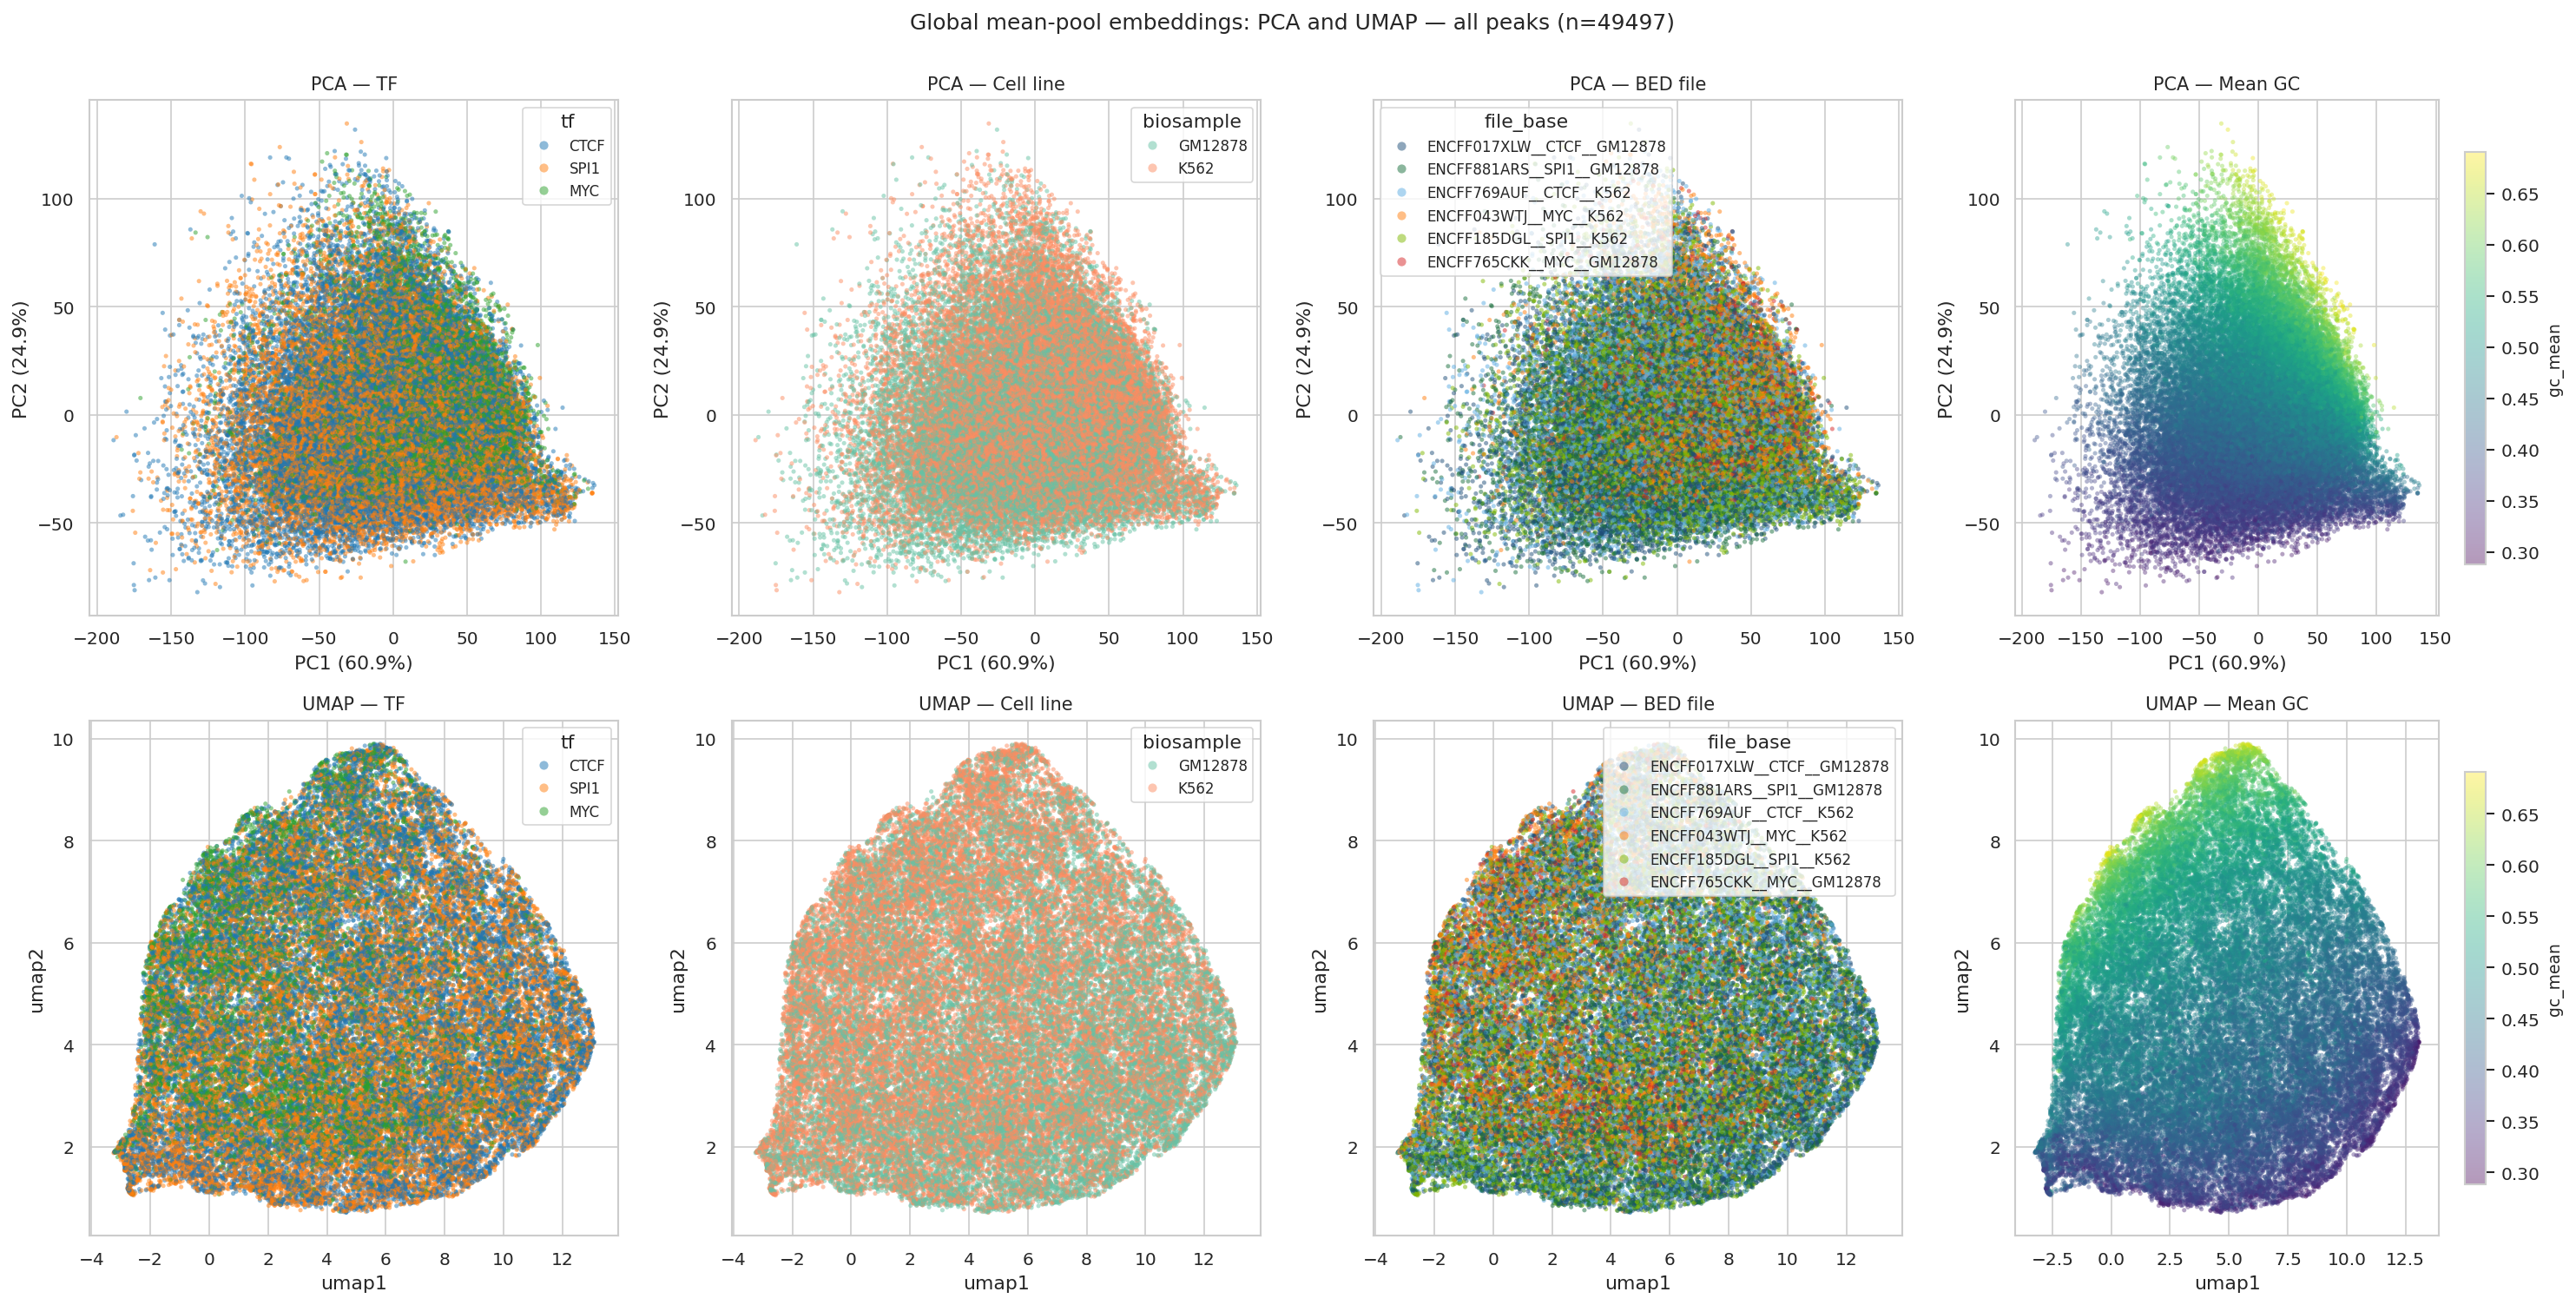
\includegraphics[width=\textwidth]{text_prace/img/block1_pca_umap_v2.png}
    % TODO: regenerate from notebook with final dataset if files change
    \caption{
        Global mean-pool PCA and UMAP of Evo~2 embeddings ($n = 49{,}497$ peaks).
        Top row: PCA scores coloured by transcription factor identity,
        cell line, BED file, and per-peak mean GC content (left to right).
        Bottom row: UMAP ($n_\text{neighbors} = 30$, $\text{min\_dist} = 0.1$)
        coloured by the same variables.
    }
    \label{fig:block1-pca-umap}
\end{figure}

The first principal component (PC1, 60.9\% of variance) is dominated by the L2 norm of the mean-pool vector \todo{compute r(PC1, L2 norm) on current dataset; expected $r \approx -0.99$}.
Variation in embedding magnitude of this scale is a representational property of the model rather than a direct reflection of input sequence content; its biological interpretation is not straightforward.

The second principal component (PC2, 24.9\% of variance) is strongly correlated with per-peak mean GC content \todo{compute r(PC2, GC) on current dataset; expected $r \approx +0.88$}, identifying GC composition as the dominant biologically interpretable axis in the global mean-pool representation.
Coloured by TF, cell line, or BED file, peaks from all groups overlap throughout the PC1--PC2 plane without visible separation (Figure~\ref{fig:block1-pca-umap}, top row).
UMAP produces a single connected manifold with a smooth GC gradient and no discrete structure attributable to TF identity, cell line, or source file (Figure~\ref{fig:block1-pca-umap}, bottom row).

Global mean pooling discards within-window positional structure by construction.
The absence of TF-discriminating signal in the dominant components of the mean-pool representation therefore does not preclude its presence in positional embeddings, which are examined in the following section.

\section{Positional structure of Evo~2 embeddings}
\label{sec:results-block2}

\subsection*{Autoregressive warm-up artefact}

\begin{figure}[htbp]
    \centering
    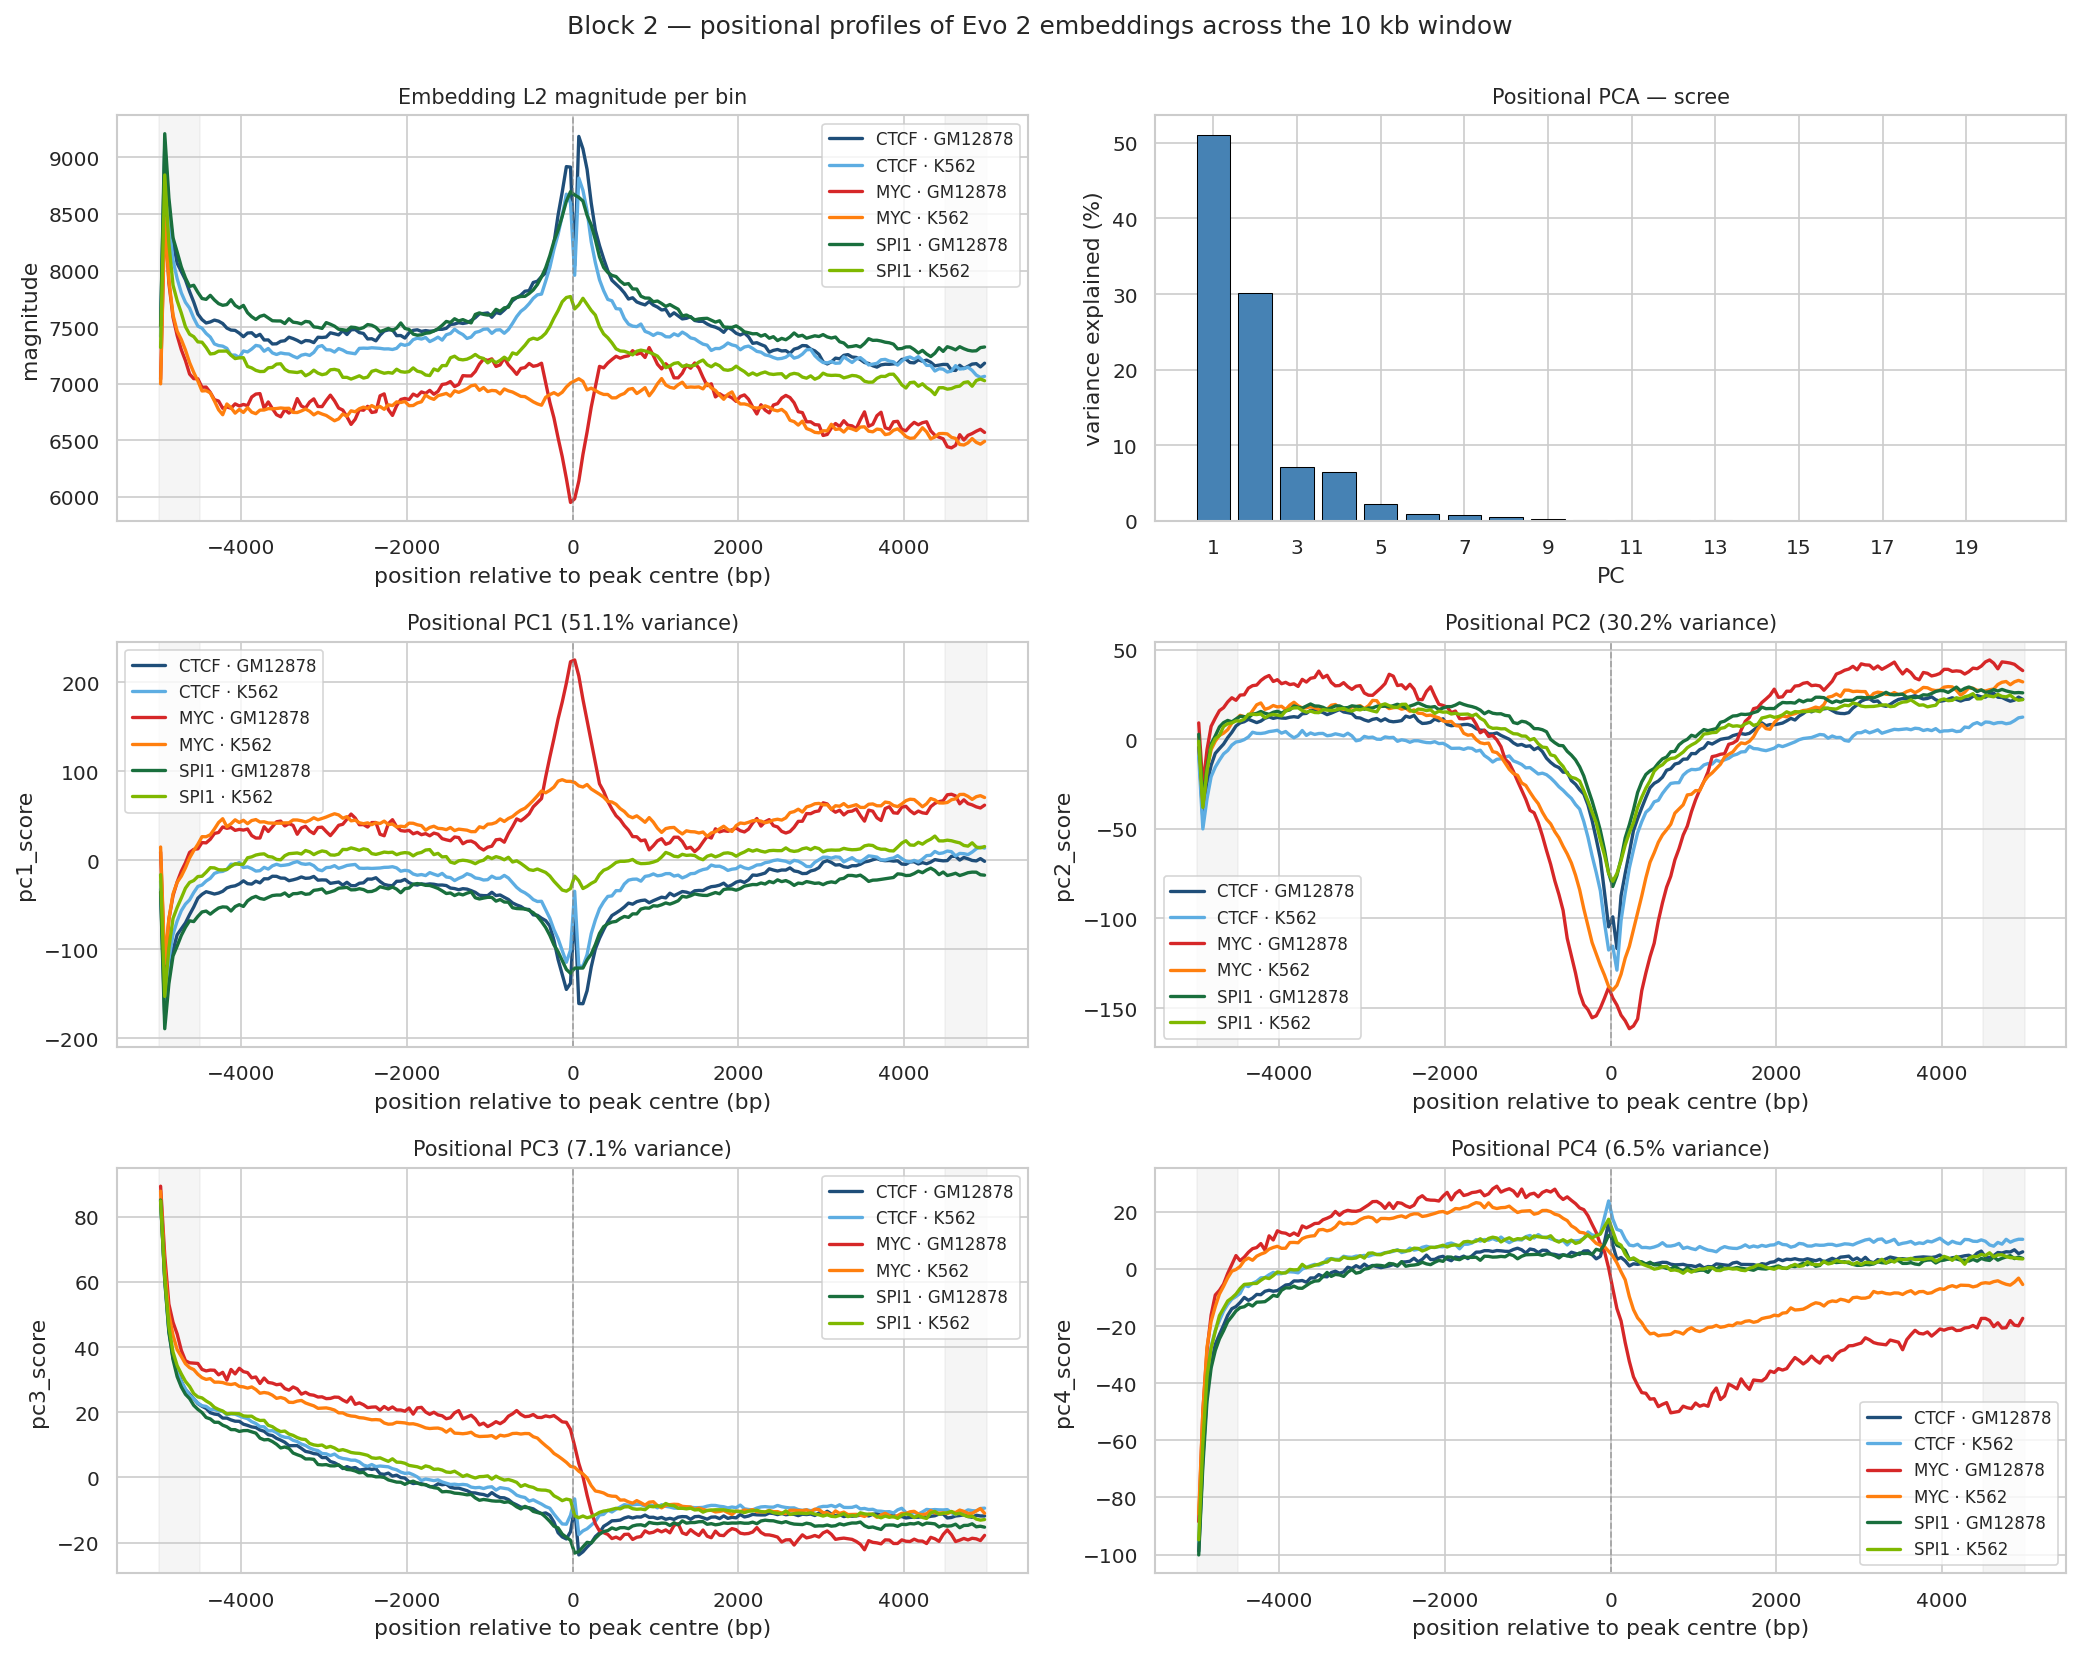
\includegraphics[width=\textwidth]{text_prace/img/block2_positional_profiles_v2.png}
    \caption{
        Positional PCA of file-level mean Evo~2 profiles, untrimmed
        (all 200 bins included in the fit).
        Top left: embedding L2 magnitude per 50~bp bin.
        Top right: scree plot.
        Rows 2--3: positional PC scores for PCs~1--4 plotted across the
        10~kb window.
        The spike confined to the leftmost bins at position
        $\approx -4750$~bp, absent at the right window edge, is the
        autoregressive warm-up artefact confirmed by the strand diagnostic
        (Section~\ref{sec:results-revcomp}).
    }
    \label{fig:block2-untrimmed}
\end{figure}

The Evo~2 7B model generates embeddings autoregressively: each token's representation is conditioned only on tokens to its left.
Tokens near the left edge of the input window therefore have little or no left context and produce activations that differ systematically from those at interior positions.
Inclusion of the BOS token during embedding (Section~\ref{sec:embeddings}) partially mitigates this effect, but does not eliminate it.
In the untrimmed positional PCA, a large spike is confined to the first approximately five bins at the left window edge ($-5000$ to $-4750$~bp), with no corresponding feature at the right edge (Figure~\ref{fig:block2-untrimmed}).
This left-to-right asymmetry is consistent with a causal warm-up artefact, as confirmed by the reverse-complement strand diagnostic described in Section~\ref{sec:results-revcomp}.
The first 15 bins (750~bp) were accordingly excluded from all subsequent positional PCA fits.

\subsection*{Reverse-complement strand diagnostic}
\label{sec:results-revcomp}

\begin{figure}[htbp]
    \centering
    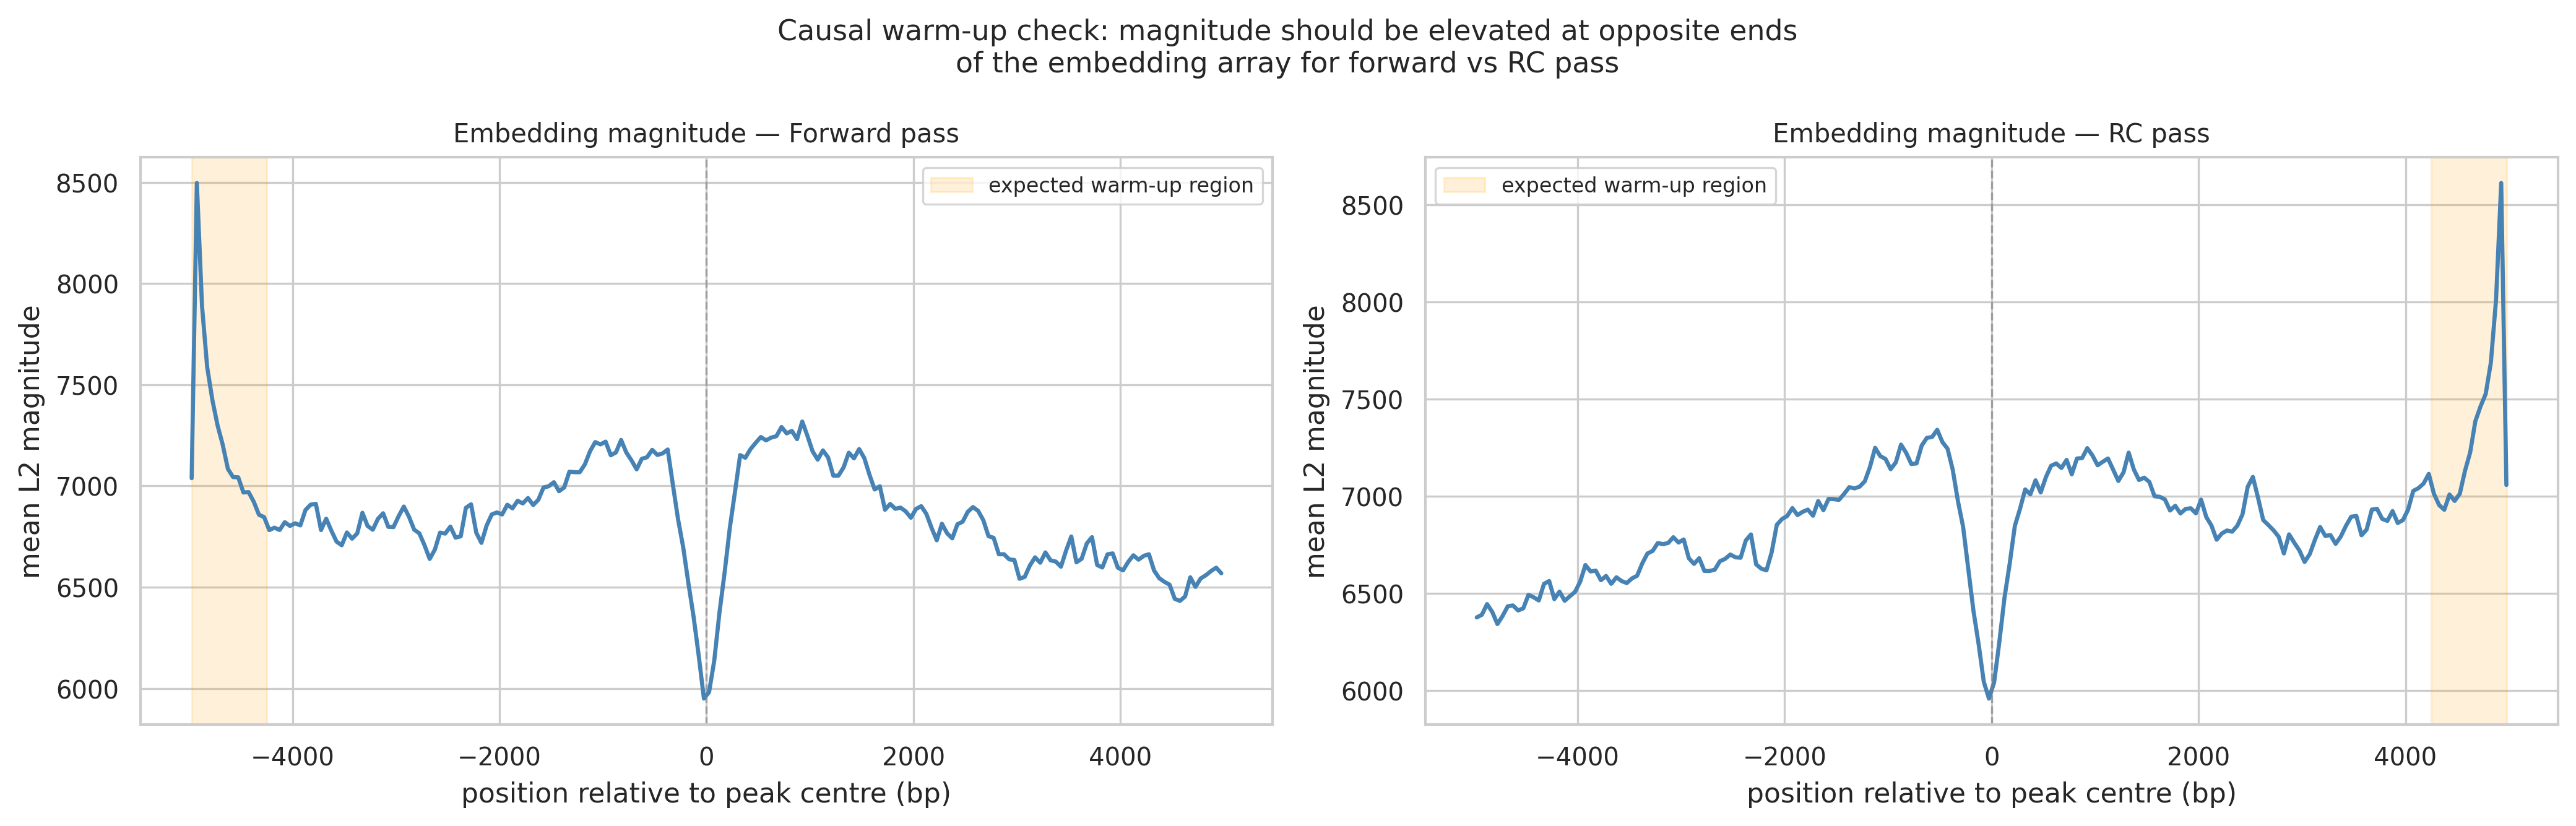
\includegraphics[width=\textwidth]{text_prace/img/revcomp_magnitude.png}
    \caption{
        Per-bin embedding L2 magnitude for the forward pass (left) and
        the reverse-complement pass (right) on MYC GM12878 peaks
        ($n = 2{,}203$).
        The RC profile is shown in genomic coordinates (bin axis flipped
        relative to model processing order).
        Orange shading marks the expected warm-up region in each pass.
        The magnitude elevation migrates from the left window edge in the
        forward pass to the right window edge in the RC pass, consistent
        with a causal autoregressive origin.
    }
    \label{fig:revcomp-magnitude}
\end{figure}

To confirm the causal origin of the left-edge magnitude elevation, the MYC GM12878 file was re-embedded with all sequences replaced by their reverse complements (Section~\ref{sec:revcomp}).
A causal warm-up artefact predicts that the elevation should migrate to the opposite end of the window when the model reads the sequence in the reverse direction.

The mean magnitude ratio of the expected warm-up region to the remaining bins was 1.059 for the forward pass (bins~0--14) and 1.073 for the RC pass (bins~185--199), with the elevation appearing at the correct genomic position in each case (Figure~\ref{fig:revcomp-magnitude}).
The symmetric migration confirms that the left-edge elevation is a consequence of autoregressive initialisation rather than a sequence property of the window edges.

As secondary checks, the GC content profiles of the RC sequences were verified to mirror the forward profiles to within $r = 0.997$ after coordinate reversal, confirming data integrity.
PC1 of a single-file trimmed positional PCA on the RC profiles was correlated with per-bin GC content at $|r| = 0.990$, compared with $|r| = 0.998$ for the forward pass, indicating that the GC--PC1 association is present regardless of strand.
The directional dinucleotide contrast profiles (AA$-$TT, CA$-$TG, AC$-$GT) computed from the RC sequences correlated with the negated and reversed forward contrast profiles at $r = 0.958$, $0.974$, and $0.969$ respectively, confirming that the asymmetry signal is strand-sensitive and inverts under strand reversal as expected for a genuinely directional sequence property.
Deviation from $r = 1.0$ is consistent with biological asymmetry of the forward profile around the peak centre.

\subsection*{Trimmed positional PCA}

\begin{figure}[htbp]
    \centering
    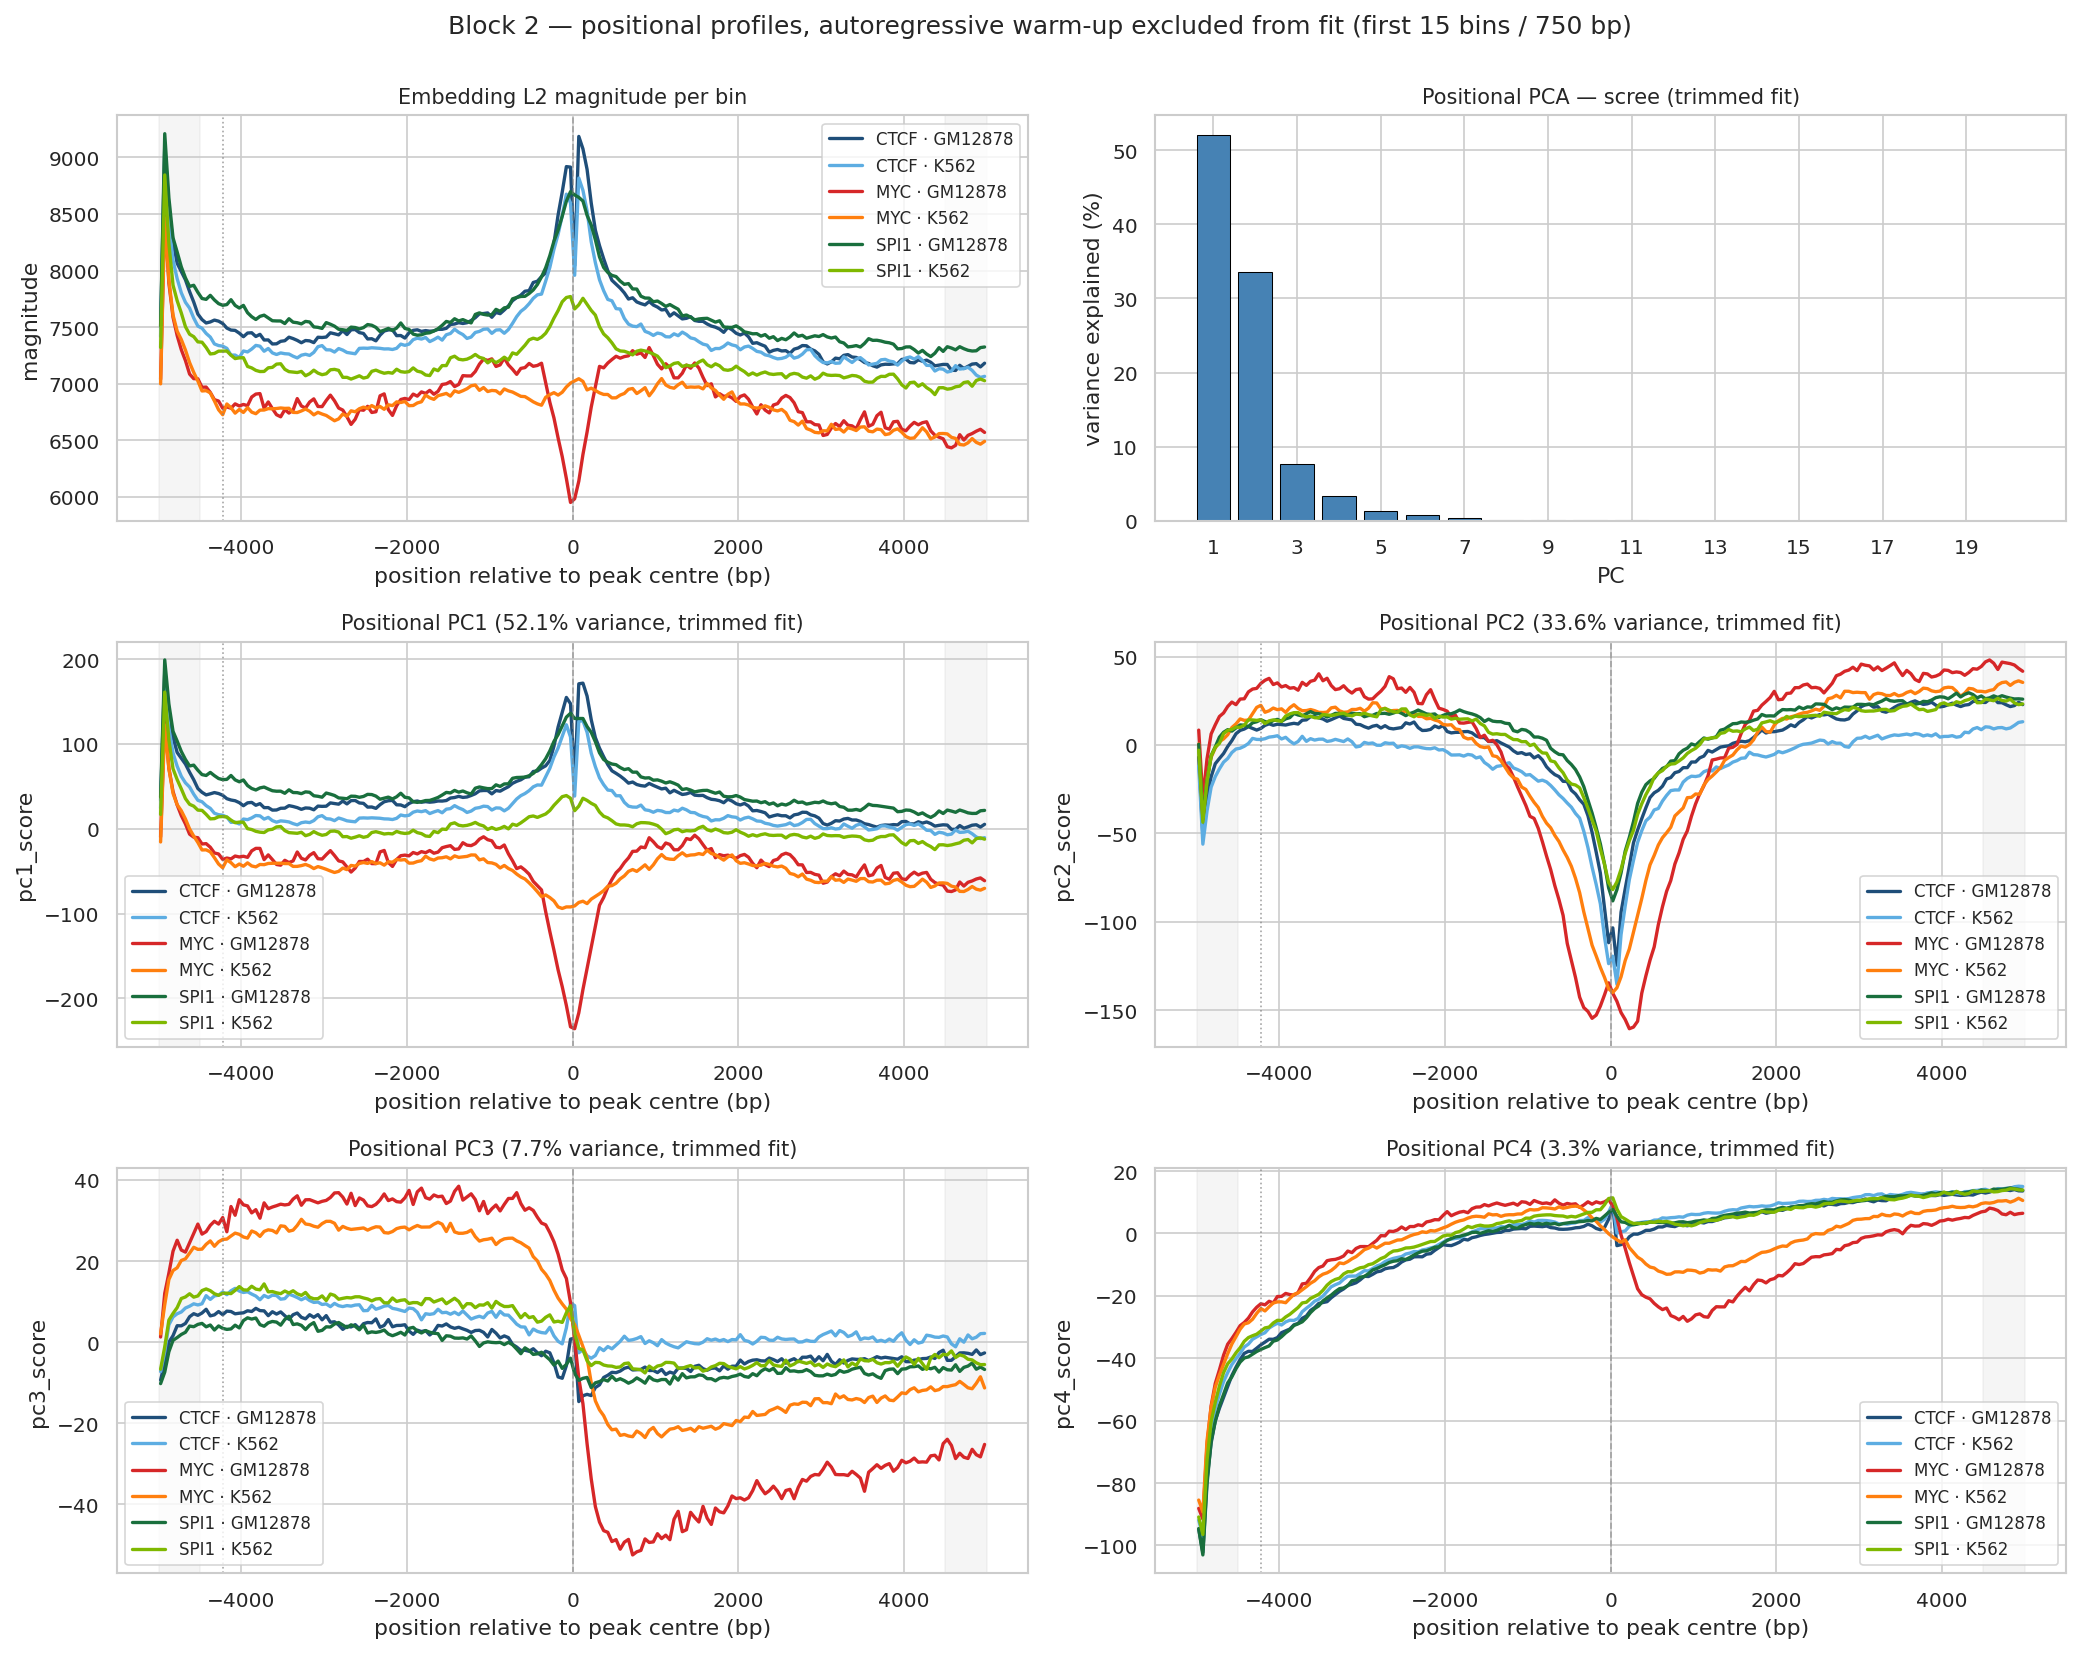
\includegraphics[width=\textwidth]{text_prace/img/block2_positional_profiles_trimmed_v2.png}
    \caption{
        Positional PCA of file-level mean Evo~2 profiles with the first
        15 bins (750~bp) excluded from the fit.
        Top left: embedding L2 magnitude per bin.
        Top right: scree (PC1 52.1\%, PC2 33.6\%, PC3 7.7\%, PC4 3.3\%).
        Rows 2--3: PC scores for PCs~1--4 across the 10~kb window.
        Shaded region: excluded warm-up bins.
        Files are labelled by TF and cell line.
    }
    \label{fig:block2-trimmed}
\end{figure}

After warm-up trimming, the leading components are PC1 (52.1\%), PC2 (33.6\%), PC3 (7.7\%), and PC4 (3.3\%) (Figure~\ref{fig:block2-trimmed}).

PC1 profiles are consistent with between-file differences in embedding magnitude: files with higher baseline magnitude show elevated scores across the window, while the two MYC files, which have the lowest baseline magnitudes, show depressed scores.
PC1 therefore does not appear to carry positional structure independent of magnitude.

PC2 displays a smooth monotonic gradient across the window, elevated at one flank and declining toward the other, shared by all six files.
The shape mirrors the per-bin GC profiles of the underlying sequences, implicating GC positional content as the primary driver of PC2; this is examined further in the L2-normalised analysis below.

PC3 (7.7\%) separates the two MYC files from CTCF and SPI1.
Both MYC~GM12878 and MYC~K562 display an antisymmetric profile around the peak centre — elevated on one flank and depressed on the other, with the transition near position 0 — while CTCF and SPI1 files remain near zero across the window.
CTCF and SPI1 are not distinguished from each other in any of the four leading components.

\subsection*{L2-normalised positional PCA}

\begin{figure}[htbp]
    \centering
    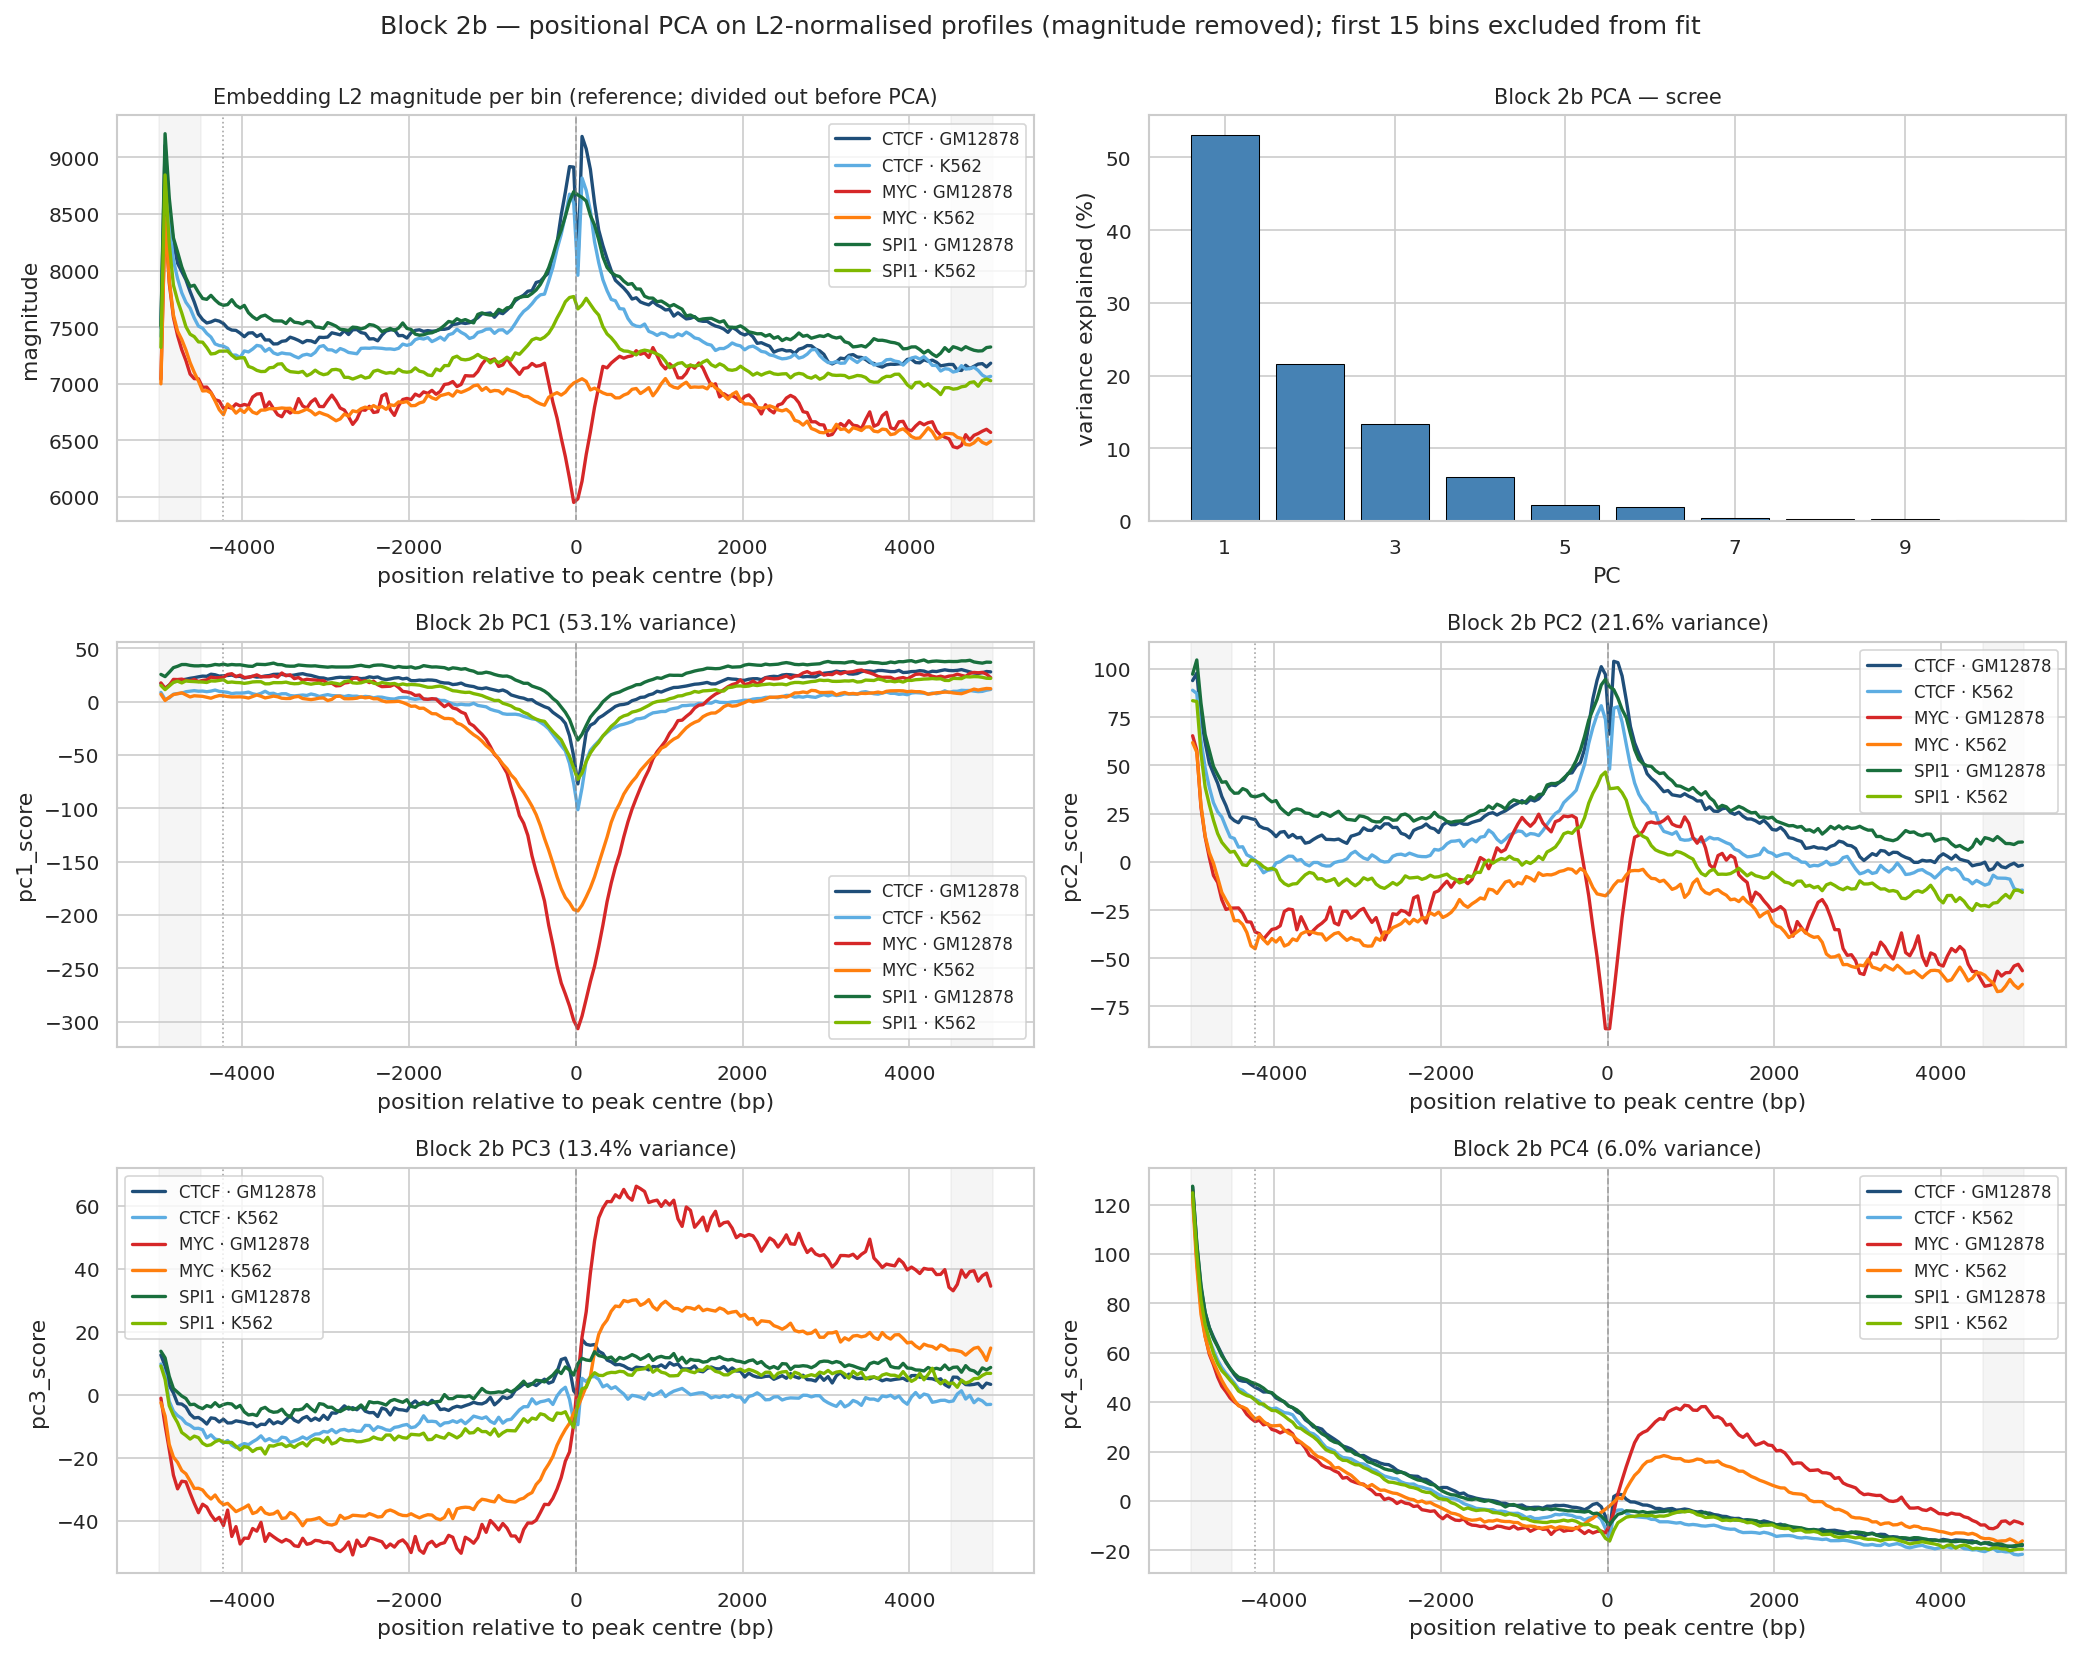
\includegraphics[width=\textwidth]{text_prace/img/block2b_positional_l2norm_v2.png}
    \caption{
        Positional PCA after L2 row-normalisation of file-mean profiles
        (embedding magnitude removed before fitting).
        Top left: per-bin embedding L2 magnitude (reference, unchanged).
        Top right: scree (PC1 53.1\%, PC2 21.6\%, PC3 13.4\%, PC4 6.0\%).
        Rows 2--3: PC scores for PCs~1--4 across the window.
        Shaded region: excluded warm-up bins.
    }
    \label{fig:block2b-l2norm}
\end{figure}

To isolate directional variation in the file-mean profiles independently of overall activation magnitude, each (file, bin) row of the stacked array was L2-normalised to unit length before PCA (Section~\ref{sec:positional}).
Under this transformation, PC1 (53.1\%) is strongly negatively correlated with per-bin GC content across all six files (Pearson $r$ ranging from $-0.957$ to $-0.997$), confirming that GC positional content is the dominant source of directional variation in Evo~2 positional embeddings once magnitude differences are removed.
PC2 (21.6\%) is strongly positively correlated with per-bin embedding magnitude across all files ($r$ from $+0.940$ to $+0.996$), indicating that the magnitude gradient along the window — itself a property of the autoregressive forward pass — is the second directional axis after GC.

PC3 (13.4\%) displays an antisymmetric profile in both MYC files: scores are elevated on one flank and depressed on the other, with the transition near the peak centre, mirroring the PC3 signal in the raw trimmed PCA.
CTCF and SPI1 files show reduced and variable profiles on this component.
PC3 is strongly correlated with the directional dinucleotide asymmetry contrasts reported by \citet{faltejskovaNonconsensusFlankingSequence2026a} for MYC binding sites: for MYC~GM12878, Pearson $r = -0.971$, $-0.982$, $-0.985$ for the AA$-$TT, CA$-$TG, and AC$-$GT contrasts respectively; for MYC~K562, $r = -0.968$, $-0.978$, $-0.976$.
The corresponding correlations for CTCF and SPI1 files are substantially weaker (CTCF $|r| \leq 0.58$; SPI1 $|r| \leq 0.90$).
The PC3 signal in MYC is therefore aligned with the directional dinucleotide asymmetry known to characterise kilobase-scale flanks of MYC binding sites, and its persistence after L2 normalisation indicates it is not attributable to differences in embedding magnitude.
Whether the Evo~2 representation encodes this dinucleotide pattern specifically, or a correlated sequence feature, cannot be determined from the present analysis.

\shorthandon{-} 
%%%%%%%%%%%%%%%%%%%%%%%%%%%%%%%%%%%%

